
\chapter{Compact Object in Globular Clusters}
\thispagestyle{fancy}

\section{Location, Location, Location}

Important in real estate, but also seems to be an important factor to take into account when studying compact objects in binary system. It seems that, like with people, where you were born plays a role on your formation and evolution. This is true for cataclysmic variables (CVs), the kind of compact binary system that we will explore in more detail in the present work. Our goal is to try to understand the formation of these kind of systems when they are formed in a crowded and high density environment (like in a cluster of stars), and when you give them enough time to evolve and interact with other stars (like in a globular cluster). \\ 

Now that we defined our broad goal let's take a step back and explore in more details what are compact objects, their different types, and the different ways they can interact with each other and other types of stars (next section \ref{sec:co}. That section will lead us to the discussion of where and how we expect to find them, and what can we learn by studying them in the different environment where they form (sections \ref{sec:gc} and \ref{sec:spec}).

\section{Compact Objects or Stellar remnants}\label{sec:co}

Compact object, as their name suggest, are very massive and dense objects formed from the remains of a dying stars; hence their other name stellar remnants. They come in three different flavors, each following a different formation mechanism that is mainly determined by the mass of the progenitor star (do I need a reference for this?). The different types are neutron stars, black holes and white dwarfs. Besides these three, other possible exotic types of stars have been proposed. Including quark stars, boson stars and Thorne-Zytkow objects. These will not be discussed in this work as there is still lack of physical observational evidence on there existence. The reader is refer to the following references if so inclined to know more about these particular kind of proposed stars. (Find references for exotic stars).


%\subsection{Neutron Stars: Nature's lighthouses}\label{sec:ns}
\subsection{Neutron Stars}\label{sec:ns}

Neutron stars, first proposed in 1934 by Baade and Zwicky,  are stars where the sustaining force is produced by the degeneracy pressure between neutrons. (ref. Baade and Zqicky '34). These stars are produced from the gravitational collapse of a massive star (> 8 M$_\odot$)(ref for mass range), at the end of its life. The massive supernova produced by this collapse, lefts behind a dense and massive core. A core of a couple of kilometers in radius (exact number?), but sustaining possible up to 2 Solar mas (ref for max observed NS or Oppenhiemr limit). They are mainly  composed of neutrons and a thin atmosphere of a few cm of Hydrogen and other heavier elements (ref for NS atmosphere models). We have come a long way since the first proposition of their existence, but there still a lot of  uncertainty on their interior and a lot of conflicting models. Since we have had observational evidence on their existence (ref first observational evidence, maybe first pulsar PSR B1919+21?) efforts have been done to constraint the different physical models. Figure~\ref{fig:nsmod} shows a visual summary of the different models proposed. There are many ways that we can observationally constraint these models, spectroscopy being one of them. Spectroscopy is still the gold standard for observational astronomy of the electromagnetic radiation. The advantages of using spectroscopy to study compact objects is discussed later in section~\ref{sec:spec}. The focus of the section is on the advantages of spectroscopy for the study of white dwarfs, but the same applies to systems with a neutron star object. The details on the future plans on how to use MUSE data to constraints such models of a neutron stars are left for the future work section (\ref{sec:futur}).\\


It is important to note that these dense objects are expected to be formed as isolated objects, but are also known to be found in binary system. They can interact with other compact objects and main sequence (MS) stars~\footnote{Main sequence stars are those that for millions of years spend their time burning hydrogen at their cores.}. The impatience reader can skip to sec~\ref{sec:cb} for more details on the kind of binary systems in which we expect to find a neutron star. We now continue with our discussion of other types of compact object. The next in line being probably the one who gets more attention out of all: black holes



\subsection{Black Holes}\label{sec:bh}

The term was coined by John Wheeler in 1968 (reference for the term), but the idea about an object so massive that don't even light could escape have been around for centuries (Ref. for Laplace 1795). Like neutron stars they are the fate of really massive stars. In this case even more massive objects were no known force can fight gravitational attraction. 

These are fascinating objects and a lot can be said about them. They have been extensively studied and indirectly observed across the electromagnetic spectrum, and most recently with gravitational waves observatories (LIGO ref). But we won't discussed them anymore in here. They will be briefly mentioned again when discussing the population of compact objects expected to be found in the dense regions of our galaxy halo (globular clusters~sec~\ref{sec:cogc}. 

Now we pass to the last type of known compact object: white dwarfs. They will be the subject of most of the rest of this report. 

\subsection[White Dwarfs]{White Dwarfs: The poor star's fate}\label{sec:wd} 

White dwarfs are by far the most common type of compact objects. It is the fate of most main sequence stars when they burn all the available hydrogen in their cores (give percentage and citation). This will also be the ending of our own Sun several billions years from now. Something so common, yet so unknown. It is true that thanks to the development of quantum mechanics and multi-wavelength observation of these objects (gravitational waves observation of these objects will have to wait until the eLISA mission) we have learned a great deal about them, but still a lot of uncertainty surrounds them. Specially on their formation and evolution when in a binary systems. That is the main motivation behind this work. But now lets take a step back and defined precisely what are white dwarfs and briefly discussed what we do know about them. 

White dwarfs, like neutron stars, are supported by the degeneracy pressure. In the case of a white dwarfs this pressure is due to the electrons and not the neutrons. But unlike neutron stars the progenitor star (a MS star of > 8 M$_\odot$) has a more complex history leading to the formation of the compact object. A qualitatively picture of the evolution of the progenitor star as it "moves" through the Hertzsprung-Russell (HR) diagram\footnote{ The Hertzsprung-Russell or HR diagram is basically a log-log plot of luminosity $L$ vs. effective temperature. This is widely use in astronomy.} is shown in figure~\ref{fig:hrwd}. The field of stellar evolution is an active and complex area of research and the reader is invited to read $---------$ for a more detail review. For us the details of the evolution of the progenitor star of the white dwarf is not so important, but it is a good way to introduce the HR diagram. The HR diagram is an useful tool and the names of the different regions indicated in the HR diagram presented in figure~\ref{fig:hrwd} is something to keep in mind for the rest of this report.  

\begin{figure}[]
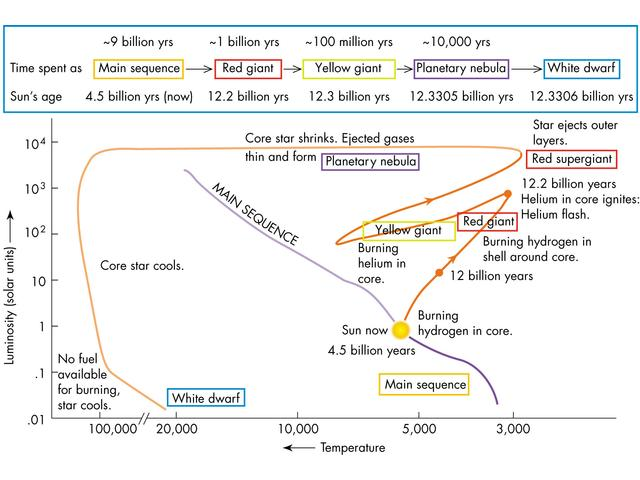
\includegraphics[scale=3]{assets/images/starevol.jpg}
\caption{Evolution Sun-like star to white dwarf. Source: The sloan digital sky server data \protect\url{http://skyserver.sdss.org/dr1/en/astro/stars/stars.asp}}
\label{fig:hrwd}
\end{figure}

Continuing our comparison between the different compact objects, it only left to say that white dwarfs too are expected to be found in binary systems. This is the topic of the next section.  


very energetic events that result from i

Exotic interacting binaries with collapsed stars are among the most powerful energy sources in the Universe, outshining their host galaxies. Interacting binaries are a rich laboratory for a wide variety of astrophysical phenomena.



Mention violente mechanism as novae anddwarf novae. Study the nature of accretion. An universal phenomena present at many scales. 


\subsection[Compact Binaries]{Compact Binaries: Nature's "Death Stars"}\label{sec:cb}

where we will explore part of the vast compact binary zoo.


In doing so we will study some of the most powerful events in the universe, result of these binary interaction of very massive objects.  



Now that we have discussed the types of compact binaries we are ready to explore how this tantalizing object can interact between themself and with other main sequence stars and form binary systems. These systems will be the object of study of the subsequence chapters.  

Accretion at different scales. An universal phenomena . 



and try to undestand what are comact obejcts 

pet's first look at what are globular clusters and see why they are the perfect place to look to study the formation and evolution of binary systems. 

WHite Dwarfs

\subsubsection{Cataclysmic Variables}

\subsubsection{LMXB}


\subsubsection{Accretion disks}


\section{Globular Clusters: A stellar nursing home}\label{sec:gc}

As we saw. We expect them to form in high density envrioment. 


What is common in both tis the accretion disks. Accretion is present in all scales. 




\subsection{NGC 6397}



\subsection{CVs in Globular clusters}\label{sec:cogc}


As usnsual we will igonre BHs. I can briefly mentioned that they are expected to be found in GC. Briefly mentioned search for spectect Intermediate BH (reference), but concentreat on CVs
For a big reviw see (big reference of GC natalie old), and relativisitc binaries is worth looking (reference mathew benacquista). A great review on CVs is kigee CVs in GC. 


I hope I have convince you by now that compact objects are a class of objecsts worth studying. There mass and densities lets us prove into physics that is still not possible with modern technology. The violent phenomena happind at the different scales is an open laboratory for high energy physics and their exoctic and excentric cores still presents a challenge for nuclear physicist. 

I also hope that I made the point that cataclysmic variables are of special interest, as they represent the fate of our own star and possibly of the vast majority of stars. These are objects that are predicted to be so common, and yet far to be completely understood. 

It should also be clear by now after the discussion on globular clusters in the last section why we would expect and search for CVs in them. But what I haven't discussed is what is our current understanding on the issue. What have we learned in years of observation and more importantly what is still to learn about them. In other words what is the motivation



Natasha paper


There are three open questions in this field:

\begin{enumerate}
        \item \textbf{Are all CVs in globlular clusters magnetic}
        \item \textbf{Where are all the primordial CVs?}
        \item \textbf{What are the periods of these white dwarfs}
        \item \textbf{Where are all the dwarf and novae?}
\end{enumerate}

\textbf{Magnetism}

The look for He II. (Emmision lines) and line ratios. 

\textbf{Primordial CVs}

Balmer series

Bright vs faint H$\alpha$, period ? (We

What hasn't been discussed is what is the current undesrtading on the topics. 
We can expect to see emmision on absoption maybe


\textbf{Period gap: Is it real?}

We need more data and sp. Emission lines can help. 


\textbf{Where are all the dwarf and novae?}

These two are violent explotion




\section{Spectroscopy: The golden standard}\label{sec:spec}

"Photometry is not enough" could have been the name of this subsection. As discussed above specific emmision and absro 
It is pretty clearn what data we need


Photometry is not enough. Prevous photometric studies (cohn, and the two vairabilty). But two answer the questions above we need spectral information. 

Emmission lines bring key information. Phenomena like accretion disk can be seen in specific wavelength (balmer series reference). Also this can help in descifering information about the nature of the compact object. Looking at the Helium as mentioned above. eIn white dwarfs for example we can look for the Helium emission lines, both He I and He II, to get more information about the magnetism and temperature of the accretion disk. He II is a sign of magnetism and He I can only be found in neutral accreting matter (ref for magnetism and accretion).  

This is not the first study of spectra in NGC 6397. Two campaings (2 Grindaly and the Edmonds paper). For other clusters also. (cite papers in talk knigge). But we are far the 15 candidates and the more than 100 predicted to exist (cohn and natasha again). 

and with this work we plan to extend the number of spectra. Limited number mainly due to the limitations on traditional slit spectroscopy. Very time consuming.  Our goal using IFU (discussed more in the methods section). Is to try to extend the population of known spectra in GC.  


%%%%%%%%%%%%%%%%%%%%%%%%%%%%%%%%%%%%%%%%%%%%%%%%%%%%%%%%%%%
%End Introduction
%
\begin{comment}
Globular clusters 
as are globular clusters.  \\

To begin I want to motivate the subject by tr

To begin I want to asnwer the question: What and what we can learn from them? and stangely enough I want to do this by asking three more questions:

\begin{enumerate}
        \item \textbf{Are all CVs in globlular clusters magnetic}
        \item \textbf{Can we see hints of primorial binaries}
        \item \textbf{}
        \item \textbf{What are the periods of these white dwarfs}
        \end{enumerate}

is the case we will look in detail in this work.  

and also seems to play a role in the formation and evolution of compact 

\section{A step back: A brief account of compact binaries}

\subsection{Compact Binaries}

\subsubsection{White Dwarfs}
\cite{harris_catalog_1996}
\end{comment}



\clearpage



\thispagestyle{empty}


